\chapter{Formato de un informe de laboratorio}
\begin{enumerate}
\item \textbf{T'itulo}
\item \textbf{Autores}
\item \textbf{Resumen}: Este �tem debe contener un breve resumen de:
  Objetivo de la Investigaci'on, Metodolog�a utilizada, teor'ias empleadas, Conclusiones.
\item \textbf{teor'ia}: En esta parte el (la) estudiante debe redactar un resumen de la teor'ia que se relaciona con el(los) objetivo(s) experimental(es) y/o indicar las variables que se infieren del (de los) objetivo(s) experimental(es). B�sicamente se debe tener en mente las preguntas �qu� medir? y/o �qu� calcular? y �para qu�?. Los verbos se escriben en tercera persona singular futuro.
\item \textbf{Material y m'etodo}: aqu'i se presenta el montaje del experimento y el �c'omo se mide aquello que se desea medir?. Se indica Adem'as la lista de materiales utilizados, se describen los instrumentos, la sensibilidad y el fondo de escala, cantidad de mediciones, etc. Un buen dibujo esquem�tico es 'util para su descripci'on. Los verbos se escriben en tercera persona singular futuro.
\item \textbf{an'alisis y Resultados}: Bajo este t�tulo se incluye la presentaci'on de los resultados del proceso de medida, organizado en
\textbf{Tablas} (su n'umero, t�tulo, definici'on de los s'imbolos de las magnitudes, unidades de medida), \textbf{Gr'aficos} (su n'umero, t�tulo, nombre de la magnitud f'isica o s'imbolo de las magnitudes y unidad de medida en cada eje, sentido en cada eje). Todos los resultados deben tener sus respectivas unidades de medida. Se deben incluir algunos c'alculos explicativos y un an'alisis cr�tico del experimento.
\item \textbf{conclusi'on(es)}: Respuesta breve y completa a lo indicado en los objetivos. Si se incluyen ecuaciones, indicar su rango de validez y su unidad de medida. Esta respuesta debe estar basada en su trabajo experimental pudiendo hacer uso de la teor'ia para apoyarse. En sus conclusiones no se aceptar�n frases especulativas sin el respaldo de datos experimentales o an'alisis expl�citos y bien fundamentados en el punto 5.
\end{enumerate}

\section{Reglas para expresar una medida y su error}

\begin{itemize}
\item Todo resultado experimental o medida hecha en el laboratorio debe ir
  acompa�ada del valor estimado del error de la medida y a continuaci'on,
  las unidades empleadas.
\item Los errores se deben indicar solamente con una �nica cifra
  significativa. �nicamente en casos excepcionales, se pueden expresar
  con una cifra y media (la segunda cifra 5 � 0)
\item La 'ultima cifra significativa en el valor de una magnitud f'isica y en
  su error, expresados en las mismas unidades, deben de corresponder al
  mismo orden de magnitud (centenas, decenas, unidades, d�cimas,
  cent�simas, etc.).
\item La identificaci'on del error de un valor experimental con el error
  cuadr'atico obtenido de $n$ medidas directas consecutivas, solamente es
  v'alido en el caso que el error cuadr'atico sea mayor que el error
  instrumental, es decir, que aquel que viene definido por la resoluci'on
  del aparato de medida.
\end{itemize}

%\chapter{Presentaci'on de datos experimentales}

\section{Tablas}
Supongamos que medimos dos magnitudes f'isicas $x$ e $y$, que est'an
vinculadas de alguna manera y que se desea descubrir c'omo se relacionan.
La primera magnitud, $x$, se mide con un instrumento distinto a la
segunda, $y$. De esta manera uno obtiene un conjunto de pares ordenados
$(x, y)$, que son la base emp'irica para establecer la relaci'on matem'atica
entre ambas variable. Independiente de c'omo sea la adquisici'on de datos,
usted poseer'a un conjunto de datos a analizar.

Una de las maneras de presentar este conjunto de datos es a trav'es de
una tabla que, en general, debe contener la siguiente informaci'on:
\begin{itemize}
\item Numeraci'on de la tabla.
\item T'itulo o descripci'on de la tabla.
\item S'imbolos de las variables usadas.
\item Unidades usadas.
\item Valores de las variables.
\item Error asociado a las medidas.
\end{itemize}

\begin{table}[h!]
\begin{center}
\begin{tabular}{|c|c|}
\hline 
Frecuencia & Voltaje \\ 
$f$, [Hertz] $\pm 1$ & $V$, [Volt] $\pm 0,2$ \\ \hline
5 & 2.6 \\ \hline 
20 & 5.0 \\ \hline
40 & 7.8 \\ \hline
60 & 11.5 \\ \hline
80 & 13.9 \\ \hline
\end{tabular}
\caption{Voltaje versus frecuencia en un circuito el'ectrico.}
\label{tab-exp1}
\end{center}
\end{table}

Sin embargo, de una tabla no se puede concluir la forma espec'ifica en que
una variable depende de la otra. T'ipicamente, un \textbf{gr'afico} de los mismos datos puede entregarnos m'as informaci'on de esta relaci'on.

\section{Gr'aficos}

La idea b'asica al construir un gr'afico es encontrar la relaci'on
matem'atica existente entre las dos variable en estudio. Al representar
gr'aficamente los valores medidos se puede visualizar la distribuci'on.
Esa distribuci'on determina la forma de la dependencia matem'atica entre
ambas variables.

Un Gr'afico debe contener la siguiente informaci'on (ver por ejemplo, la figura \ref{fig-g1}):

\begin{itemize}
\item N'umero
\item T'itulo
\item Nombre de la magnitud f'isica o s'imbolo de las magnitudes
\item Unidades de medida en cada eje
\item Si corresponde, se pueden incluir las barra de errores asociadas a cada punto.
\end{itemize}

\begin{figure}[h!]
\begin{center}
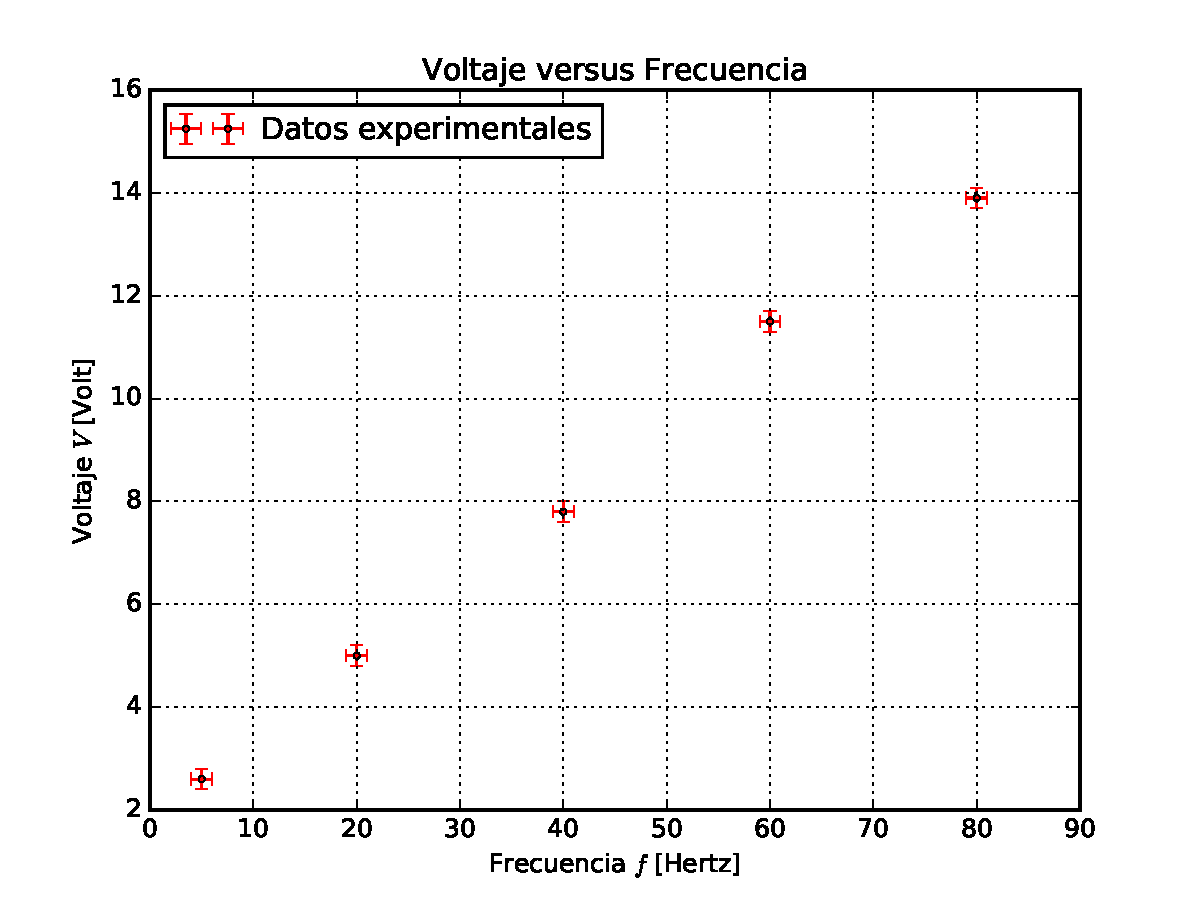
\includegraphics[width=10cm]{figs/fig-grafico-con-error.pdf}
\caption{Datos experimentales de diferencia de potencial versus frecuencia. C'odigo Python \href{https://github.com/gfrubi/Lab/blob/master/python/fig-grafico-con-error.py}{aqu\'i}.}
\end{center}
\label{fig-g1}
\end{figure}


\subsubsection{Lineal}
La idea b'asica es graficar los datos obtenidos durante el experimento (ver fig. \ref{fig-exp1}),  recopilados en la tabla \ref{tab-exp1}. En el caso particular mostrado en la fig. \ref{fig-exp1} usted puede ver que la dependencia es del tipo lineal. La mejor recta es aquella que est'a m'as cerca de todos los puntos a la vez, aunque no tiene necesariamente que pasar por todos los puntos, m'as a'un, \textit{puede no pasar por ninguno de ellos}.

La ecuaci'on de la recta esta dada por $y=mx+n$, donde 
\begin{equation}
m=\frac{\Delta V}{\Delta f}=0,5,
\end{equation}
\begin{equation}
n=V-mf=2,0-0,15\times 0=2,0,
\end{equation}
\begin{equation}
V(f)=0,15 f +2,0, \qquad 5<f<80.
\end{equation}
\begin{figure}[h!]
\begin{center}
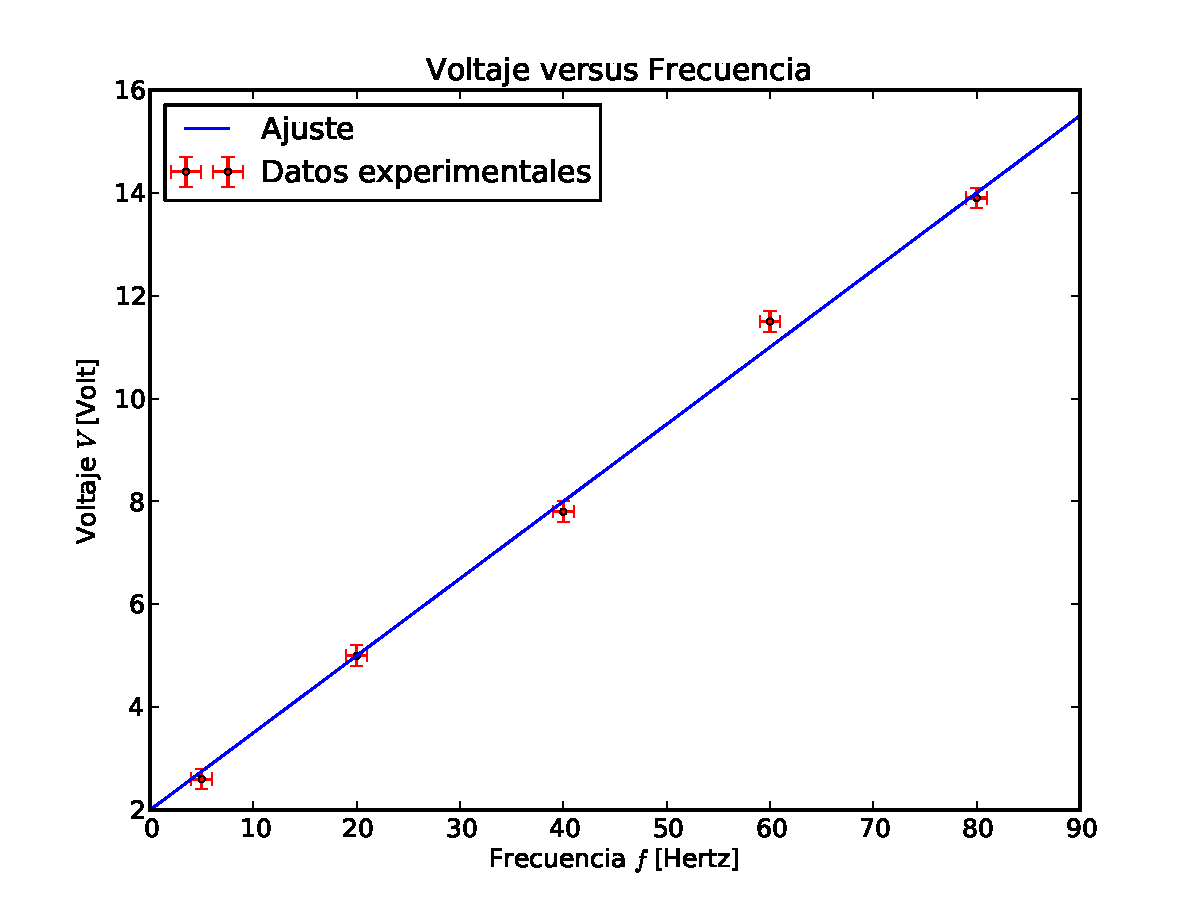
\includegraphics[width=10cm]{figs/fig-ajuste-lineal.pdf}
\caption{Voltaje versus frecuencia en un circuito el'ectrico y ajuste lineal.  C'odigo Python \href{https://github.com/gfrubi/Lab/blob/master/python/fig-ajuste-lineal.py}{aqu\'i}.}
\end{center}
\label{fig-exp1}
\end{figure}

\subsubsection{Log-Log}
En esta escala usted encuentra que los espacios est'an divididos en segmentos desiguales en ambas direcciones. En cada direcci'on las divisiones igualmente espaciadas son potencias de 10, correspondiendo a los ciclos que se repiten.

De manera an'aloga al caso anterior, se grafican los datos recopilados durante la experiencia (ver fig. \ref{fig-exp2}), que se encuentran ordenados en la Tabla \ref{tab-exp2}. 

\begin{table}[h!]
\begin{center}
\begin{tabular}{|c|c|}
\hline 
Fuerza & Deformaci'on \\ 
$F$, [N] & $L$, [mm] $\pm 0.2$ \\ \hline
$5.0\pm 0.3$ & 1.0 \\ \hline 
$16\pm 1$ & 2.0 \\ \hline
$80\pm 1$ & 4.0 \\ \hline
$160\pm 5$ & 6.0 \\ \hline
$400\pm 5$ & 9.8\\ \hline
\end{tabular}
\caption{Fuerza aplicada sobre una barra met'alica.}
\label{tab-exp2}
\end{center}
\end{table}
\begin{figure}[h!]
\begin{center}
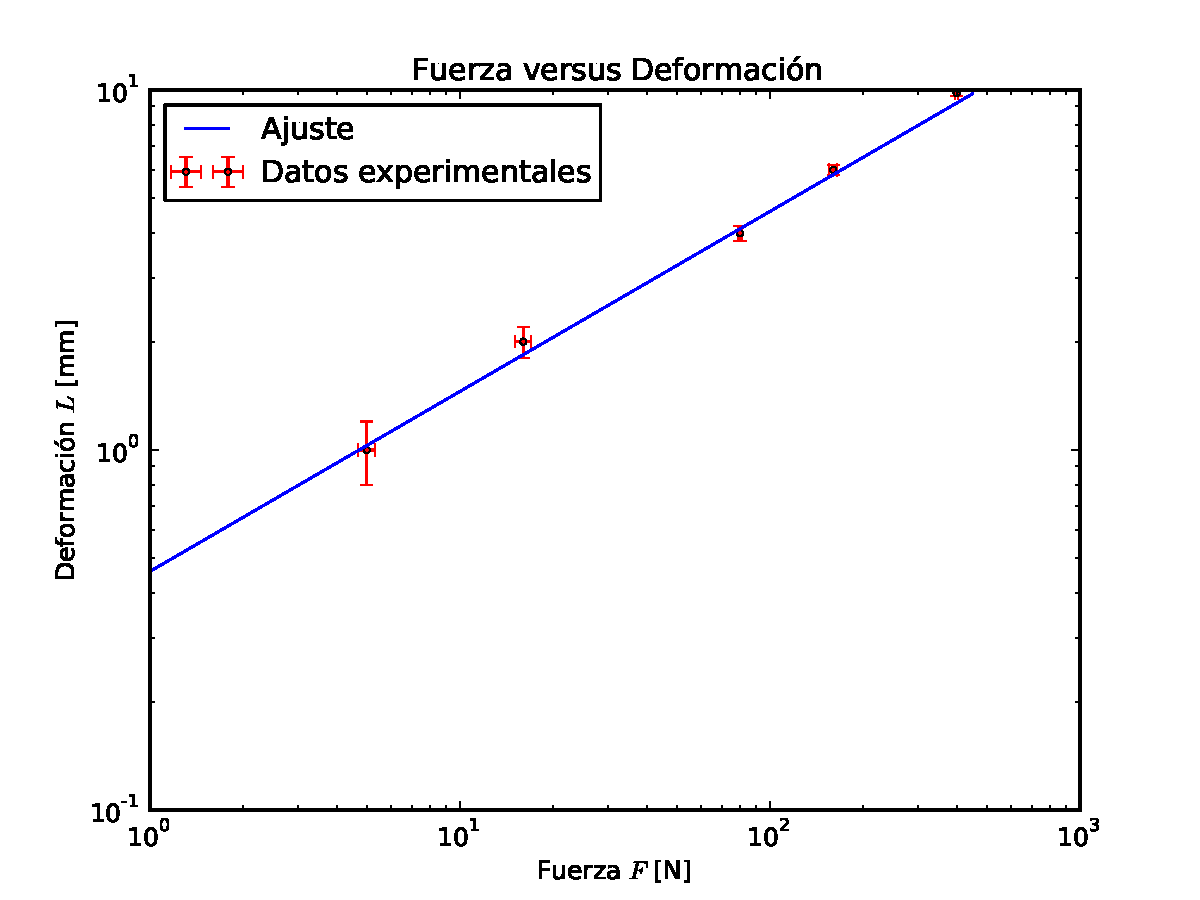
\includegraphics[width=10cm]{figs/fig-ajuste-log-log.pdf}
\caption{Fuerza aplicada sobre una barra met'alica. Gr'afico log-log y ajuste. C'odigo Python \href{https://github.com/gfrubi/Lab/blob/master/python/fig-ajuste-log-log.py}{aqu\'i}.}
\end{center}
\label{fig-exp2}
\end{figure}

La ecuaci'on de la recta para este caso, est'a dada por:
\begin{equation}\label{logLlogF}
\log(L)=m\log(F)+\log(A),
\end{equation}
donde $m$ es la pendiente, definida como 
\begin{equation}
m=\frac{\Delta\log(L)}{\Delta\log(F)}=\frac{\log(3)-\log(2)}{\log(40)-\log(18)}=0,508.
\end{equation}
Para determinar la constante $A$, evaluamos en un punto sobre la recta:
\begin{equation}
\log(L)=0,508\log(F)+\log(A).
\end{equation}
Evaluando en $F=1$, encontramos
\begin{align}
\log(L) &= 0,508\log(1)+\log(A) \\
&= \log(A),
\end{align}
y por lo tanto $L=A\approx 0,46$. Por lo tanto, muestro ajute es en general de la forma \eqref{logLlogF}, que es equivalente a
\begin{equation}
L=A\times F^m,
\end{equation}
de modo que en este caso tendr'iamos
\begin{equation}
L\approx (0,46)\times F^{0,5} \text{ mm}, \qquad 5\le F\le 400.
\end{equation}

\subsubsection{Semilog}
En este caso usted encuentra que en una direcci'on las divisiones son desiguales como en la situaci'on anterior y en la otra direcci'on las divisiones de los espacios est'an igualmente distribuidos.

Procediendo como en los casos anteriores, ordenamos los datos experimentales en la Tabla \ref{tab-exp3} y luego se grafican (ver fig. \ref{fig-exp3}),  donde se aprecia una dependencia lineal.
\begin{table}[h!]
\begin{center}
\begin{tabular}{|c|c|}
\hline 
Tiempo & Carga el'ectrica \\ 
$t$, [ms] $\pm 0.1$ & $Q$, [mC] $\pm 0.002$ \\ \hline
$4.0$ & $0.780$ \\ \hline 
$8.0$ & $0.260$ \\ \hline
$16.0$ & $0.040$ \\ \hline
$20.0$ & $0.015$ \\ \hline
$24.0\pm 5$ & $0.005$\\ \hline
\end{tabular}
\caption{Carga el'ectrica y tiempo en un condensador.}
\label{tab-exp3}
\end{center}
\end{table}
\begin{figure}[h!]
\begin{center}
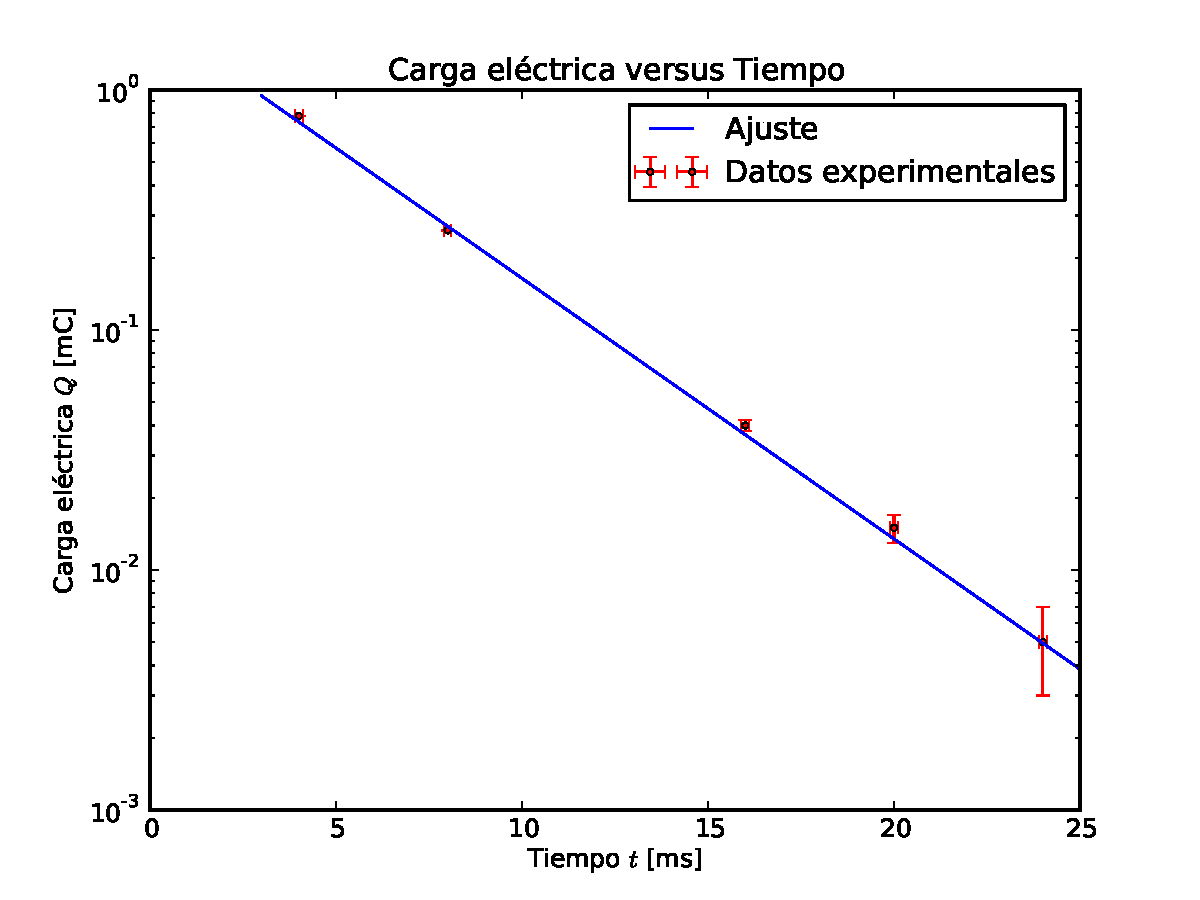
\includegraphics[width=10cm]{figs/fig-ajuste-semilog.pdf}
\caption{Carga el'ectrica y tiempo en un condensador. Gr'afico semilog y ajuste. C'odigo Python en ap'endice \ref{app-6}.}
\end{center}
\label{fig-exp3}
\end{figure}

Para el ajuste de una recta, se tiene
\begin{equation}\label{logQt}
\log(Q)=mt+\log(A), \qquad \Leftrightarrow \qquad Q=A\times 10^{mt}
\end{equation}
\begin{equation}
m=\frac{\log(0,0022)-\log(0,046)}{(27-15)\times 10^{-3}}\approx -110
\end{equation}
En muchas ocasiones ser'a conveniente expresar la funci'on ajustada usando base $e$:

\paragraph{Repaso: } 
\begin{equation}
y=e^x \quad \Rightarrow\quad \ln y=x, \quad \log(y)=x\log(e),
\end{equation}
\begin{equation}
\frac{\log(y)}{\ln(y)}=\log(e) \quad \Rightarrow\quad \log(y)=\ln(y)\log(e).
\end{equation}
Aplicando esta propiedad a la ecuaci'on $Q(t)$, encontramos
\begin{equation}
m=\frac{\log(y_{\rm f})-\log(y_{\rm i})}{t_{\rm f}-t_{\rm i}}=\frac{(\ln(y_{\rm f})-\ln(y_{\rm i}))\log(e)}{t_{\rm f}-t_{\rm i}},
\end{equation}
\begin{equation}
|m|=\left|\frac{\ln(y_{\rm f})-\ln(y_{\rm i})}{t_{\rm f}-t_{\rm i}}\right|\log(e)=:\frac{\log(e)}{\tau}, \quad\Rightarrow\quad \tau\approx\frac{\log(e)}{110}=\approx\frac{0,4343}{110}\approx 0,004
\end{equation}
Usando la definici'on de $\tau$ podemos reescribir la expresi'on \eqref{logQt} como
\begin{equation}
Q(t)=A\times e^{-t/\tau}.
\end{equation}
Si $t=0$ entonces $Q(0)=A\approx 2$. Por lo tanto, nuestro ajuste puede escribirse como
\begin{equation}
Q(t)\approx 2\times e^{-t/0,004}\text{ mC}, \qquad 4\text{ s}\le t\le 24 \text{ s}.
\end{equation}
Debemos hacer notar que en los tres casos mencionados para ajustar curvas, tanto para el c'alculo de la pendiente como para el punto donde la recta corta el eje vertical, se usaron los valores de la ``mejor'' recta y no (directamente) los valores experimentales.

